\section{int\_capture\_flop}
我们先从外部中断引脚开始看,看看经过哪些逻辑。以下是picoblaze的顶层接口:

\textbf{kcpsm3\_top.v}
\begin{vcode}
/*Declare begin*/
module kcpsm3(
        address,
        instruction,
        port_id,
        write_strobe,
        out_port,
        read_strobe,
        in_port,
        interrupt,
        interrupt_ack,
        reset,
        clk) ;
 
output  [9:0]   address ;
input   [17:0]  instruction ;
output  [7:0]   port_id ;
output          write_strobe, read_strobe, interrupt_ack ;
output  [7:0]   out_port ;
input   [7:0]   in_port ;
input           interrupt, reset, clk ;
/*Declare end*/
\end{vcode}


\newpage
可以从字义上理解interrupt为外部中断的入口,而interrupt\_ack为中断确认信号,interrupt首先连入int\_capture\_flop逻辑:

\textbf{int\_capture\_flop.v}
\begin{vcode}
// Interrupt capture
FDR int_capture_flop (
    .D(interrupt),
    .Q(clean_int),
    .R(internal_reset),
    .C(clk));
\end{vcode}



在Synplify的Technology View可以看到如下的图\\
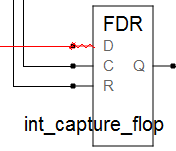
\includegraphics{int_capture_flop.png}

这个FDR是“同步复位D触发器”原语。FDR是比较好理解的,D是输入,Q是输出,R是复位,C是时钟。\\
在\verb|C:\Xilinx\12.4\ISE_DS\ISE\verilog\xeclib\unisims|下是官方给出的仿真代码。
在后面还会涉及到LUT(查找表),所以在这里先介绍一下。

\textbf{FDR}
\begin{vcode}
module FDR (Q, C, D, R);
    parameter INIT = 1'b0;
    output Q;
    reg    Q;
    input  C, D, R;
    always @(posedge C)
        if (R)
        Q <= 0;
        else
        Q <= D;
endmodule
\end{vcode}



\textbf{LUT4}
\begin{vcode}
module LUT4 (O, I0, I1, I2, I3);
    parameter INIT = 16'h0000;
    input I0, I1, I2, I3;
    output O;
    wire out0, out1, out2, out3, out;
    assign O = INIT[{I3,I2,I1,I0}];
endmodule
\end{vcode}



FDR就是一个触发器,LUT4是一个16bit的ROM结构,O是输出,I3、I2、I1、I0是地址线。

因为原语不太直观,所以在这里把\verb|int_capture_flop|改写为rtl描述。

\textbf{int\_capture\_flop\_rtl.v}
\begin{vcode}
always@(posedge clk)
begin
    if (internal_reset)
        clean_int <= 1'b0;
    else
        clean_int <= interrupt;
end
\end{vcode}



这个逻辑同步外部的中断信号。interrupt是外部中断信号,\verb|clean_int|是同步后的中断信号。 \verb|internal_reset|是PicoBlaze内部复位信号,当处理器复位的时候,\verb|internal_reset|会持续一段时间。

用原语来写有个好处就是综合的结果基本上就是你想要的电路,
但代价就是不容易维护,也不利于别人阅读。

